\section{Kerberos}

In un sistema si può aggiungere una procedura di autenticazione per ogni servizio,
ad esempio una password per accedere al sistema, una per accedere al file system,
ecc. Questa tecnica risulta essere molto scomoda, soprattutto se si utilizzano
i token. Un’alternativa consiste nell’utilizzare un’unica credenziale di
autenticazione per accedere a tutti i servizi; avere un’unica password è una
soluzione comoda ma poco robusta.
Kerberos è un \textbf{protocollo} reale che si occupa di questo problema (e non solo),
ha come obiettivo quello di garantire la segretezza, l’autenticità
(ad accesso singolo), la temporalità (le chiavi usate hanno validità limitata
per prevenire \textit{replay attack}).
Quest’ultima caratteristica viene gestita tramite
i \textbf{timestamp}. In pratica, l’accesso ad un servizio avviene tramite
“biglietto” che vale per un periodo limitato; anche se tale biglietto venisse
intercettato, può essere usato solo una volta e per un breve tempo.

\paragraph{Kerberos}
è un protocollo di autenticazione dei servizi di rete creato dal MIT che si
serve della crittografia a chiave simmetrica per autenticare gli utenti per i
servizi di rete, eliminando così la necessità di inviare le password attraverso
la rete. Ricorre ad un’unica credenziale di autenticazione per accedere a tutti
i servizi. L'autenticazione mediante Kerberos impedisce agli utenti non autorizzati
di intercettare le password inviate attraverso la rete.
Il nome Kerberos deriva da Cerbero, il cane a tre teste che sorveglia
le porte dell’Ade.\\

La maggior parte dei sistemi di rete convenzionali usa uno schema di
autenticazione basato sulle password. Quando un utente effettua una
autenticazione per accedere ad un server di rete deve fornire le credenziali.
Sfortunatamente, la trasmissione delle informazioni di autenticazione spesso
non è criptata. Per essere sicuri, la rete non deve essere accessibile
dall'esterno e tutti i computer e gli utente sulla rete devono essere fidati.
Anche una volta che una rete è collegata a Internet, non si potrà più assumere
che la rete sia sicura, in quanto qualunque aggressore che ha accesso alla rete
può intercettare le password e i nomi utente che la attraversano.
Lo scopo principale di Kerberos è quello di eliminare la trasmissione delle
informazioni di autenticazione attraverso la rete.
Il suo corretto utilizzo permette di ridurre drasticamente la possibilità di
intercettazione. Per funzionare, Kerberos deve avere possedere due requisiti:

\begin{itemize}
      \item un \textbf{timeserver} in ogni sistema dove viene utilizzato.
            I timestamp permettono di sincronizzare le macchine;
      \item ogni utente deve avere una \textbf{chiave pubblica} e una \textbf{privata}
            (una password a lungo termine).

\end{itemize}

\subsection{Come funziona ?}

L’utente, una volta entrato nella propria macchina, vuole accedere ai servizi
messi a disposizione nella rete. Supponiamo voglia raggiungere il server in basso.
Effettuato il primo accesso alla macchina, le credenziali dell’utente vengono
inviate ad uno speciale servizio centrale, il Kerberos, che ricorre essenzialmente
a due tipi di server:

\begin{itemize}
      \item \textit{Authentication Server} (\textbf{AS}\footnote{Ricordarsi che
                  AS non sta per
                  \textit{Autonomous System} !}),
            che ha lo scopo di autenticare l’user;
      \item \textit{Ticket-Granting Server} (\textbf{TGS}), che a seconda dell’user,
            gli assegna i diritti per compiere determinate azioni;
\end{itemize}

\begin{figure}[H]
      \centering
      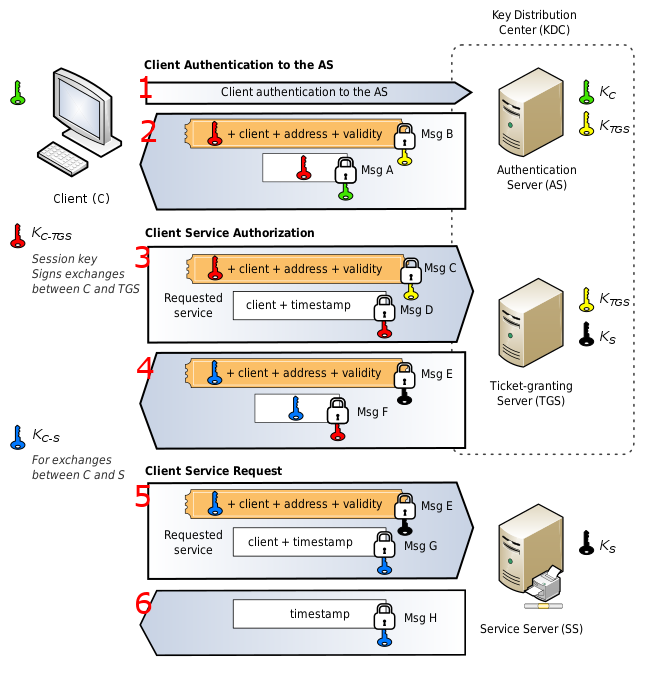
\includegraphics[width=10cm, keepaspectratio]{capitoli/autenticazione/imgs/kerberos1.png}
      \caption{Schema di funzionamento del protocollo Kerberos.}
\end{figure}

\begin{enumerate}
      \item L’utente si connette con le proprie credenziali alla workstation e
            queste vengono passate al Kerberos;
      \item AS verifica il diritto di accesso dell’utente, ricercando una
            corrispondenza nel database. Se il confronto ha esito positivo, AS
            assegna all’user un ticket e una session key.
            Il ticket verrà poi passato al TGS per richiedere i servizi, mentre
            la chiave permette di codificare le sue richieste, sempre poste al TGS.
            Entrambe le informazioni vengono criptate;
      \item L’utente a questo punto vuole utilizzare un certo servizio.
            La workstation richiede all'utente la password e la utilizza per
            decrittografare il messaggio in arrivo, quindi invia ticket e
            autenticatore
            (che contiene il nome, la rete, l'indirizzo e l'ora dell'utente) a TGS;
      \item TGS decripta il ticket e l'autenticatore, verifica se esso ha il
            diritto o meno ad utilizzare una certa risorsa e crea il ticket
            specifico per il servizio richiesto. La comunicazione tra utente e
            TGS avviene solo grazie alla session key che la codifica;
      \item La workstation manda ticket e autenticatore al server;
      \item Il server verifica il match tra ticket ed autenticatore e permette
            l’accesso al servizio. Se
            viene richiesta una mutua autenticazione, il server ritorna un
            autenticatore.
\end{enumerate}

È importante notare che l’utente può utilizzare il ticket finché esso risulta
ancora valido, il che può accadere anche per più tentativi di richiesta al servizio.
Per un servizio diverso mai utilizzato, deve ripercorrere il medesimo processo.\\

Kerberos opera fondamentalmente in \textbf{3 fasi} e ognuna di queste fornisce
le credenziali per la successiva:

\begin{figure}[H]
      \centering
      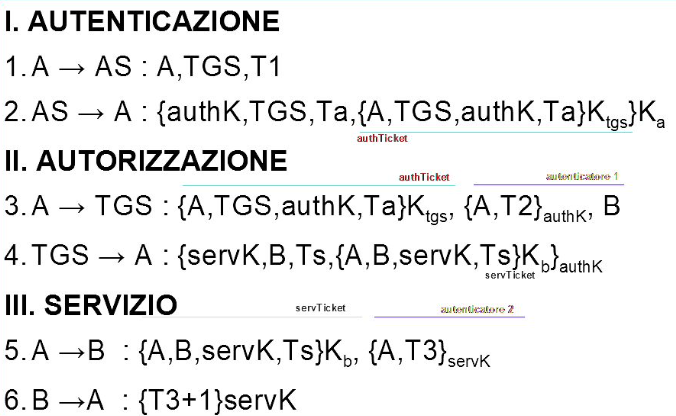
\includegraphics[width=10cm]{capitoli/autenticazione/imgs/kerberos2.png}
\end{figure}

\begin{enumerate}
      \item All’autenticazione si ottiene \verb|authK| e \verb|authTicket|.
            Il primo per autenticarsi e rendere
            riservata la trasmissione con il TGS, il secondo per ottenere
            il servizio del TGS;
      \item Nell’autorizzazione da parte del TGS, si ottiene \verb|servK| e
            \verb|servTicket|, da presentare per il
            server richiesto;
      \item Il servizio conferma poi la richiesta.
\end{enumerate}

\verb|authK| e \verb|servK| sono chiavi simmetriche, in quanto possono essere
usate sia per criptare che per decriptare. Ogni chiave di sessione ha una
propria durata.
Chiaramente quella della \verb|servK| è minore rispetto a quella
della \verb|authK|.

\subsection{Nel dettaglio}

\textit{A} è l’utente che richiede il servizio \textit{B}.
\textit{A} si autentica all’AS ad un certo tempo \verb|T1|
(\textit{messaggio 1}). Se l’utente non è registrato tra quelli del dominio,
non viene preso in considerazione. Se invece è autorizzato, si verifica grazie
al ticket a quale TGS vuole rivolgersi.
\textit{A} per autenticarsi ha inviato solo il nome dell’utente, però l’AS fa
una challenge: invia ad \textit{A} un’informazione e se l’utente è
effettivamente chi dice di essere, allora saprà decifrarla con la sua chiave.
\textit{A} apre il pacchetto con la chiave privata (\textit{messaggio 2}).
All’interno trova:

\begin{itemize}
      \item un \verb|authTicket| codificato con la chiave di TGS e quindi non può
            aprirlo;
      \item la conferma del fatto che il TGS è disponibile a ricevere le sue
            richieste;
      \item il tempo \verb|Ta| in cui AS ha inviato la risposta;
      \item \verb|authK|, cioè una chiave di sessione che vale per un certo periodo di
            tempo (stabilito dalla configurazione) a partire da \verb|Ta|;
\end{itemize}

All'interno del \textit{messaggio 3} abbiamo:

\begin{itemize}
      \item ticket ricevuto dall'AS, anche se non sa cos’è;
      \item il suo nome e \verb|T2| che corrisponde all’istante in cui viene
            inviato il pacchetto. Il tutto è
            codificato da \verb|authK|;
      \item nome del servizio a cui vuole accedere, cioè \textit{B};
\end{itemize}

Il fatto di inviare \textit{A} e \verb|authK| permette di autenticarsi con il TGS.
\verb|authK| è stata inviata da AS e poiché TGS si fida di AS, riesco ad aprire
il messaggio \verb|{A, T2}| dell’autenticatore 1. Il messaggio è chiaramente
scritto da \textit{A} e la conferma arriva dal fatto che \textit{A} è scritto
anche fuori in \verb|authTicket| e l’\verb|authK| è stato condiviso da AS
con \textit{A}. A questo punto \textit{A} è autenticato.
Se il \textit{messaggio 3} fosse stato inviato al TGS sbagliato, al richiesta
non verrebbe presa in considerazione. \verb|Ta| permette di capire se \verb|authK|
è ancora valida.
Il TGS verifica se \textit{A} ha il diritto di utilizzare \textit{B}. Se così è,
viene autorizzato con l’invio del \textit{messaggio 4}:

\begin{itemize}
      \item È criptato con \verb|authK| e solo \textit{A} può aprirlo.
            Si usa \verb|authK| perché altrimenti si potrebbe usare il ticket al
            posto di \textit{A};
      \item grazie ad \verb|authK| siamo sicuri che il messaggio viene aperto
            da TGS ed \textit{A} perché la chiave è condivisa
            (ci sono sia confidenzialità che autenticazione);
      \item TGS verifica che ci sia scritto \textit{B}, altrimenti il messaggio
            viene eliminato. \textit{A} è autorizzato ad utilizzare \textit{B}
            a partire dal momento \verb|Ts|
            (momento in cui TGS invia il messaggio ad \textit{A});
      \item la chiave di sessione \verb|servK| ha una certa durata a partire
            da \verb|Ts|. È la session key da utilizzare con il servizio;
\end{itemize}

Il \textit{messaggio 5} che va da \textit{A} a \textit{B} invece:

\begin{itemize}
      \item prende il ticket \verb|servTicket| che gli ha dato il
            server precedente;
      \item \textit{A} per autenticarsi con \textit{B} scrive \verb|{A, T3}|
            codificato con \verb|servK|. Viene decodificato
            autenticatore 2 e si ha la certezza che \textit{A} ha inviato il
            messaggio. Se \verb|T3| è troppo distante da \verb|Ts|,
            il messaggio perde di validità. Anche in questo
            caso \textit{A}, \textit{B} e TGS conoscono la durata delle chiavi
            di sessione;
      \item \verb|Kb| è una chiave condivisa tra \textit{B}, TGS e AS
\end{itemize}

Il \textit{messaggio 6} viene inviato come risposta al fatto che la richiesta è
stata accettata:

\begin{itemize}
      \item \verb|{T3+1}| è criptato con \verb|servK|,
            questo per evitare dei replay attack;
\end{itemize}

È doveroso notare che non sono solo le chiavi ad essere simmetriche,
anche lo stesso protocollo lo è.
Questa versione di Kerberos è la 4, che attualmente non viene utilizzata.

\subsection{Gestione delle Chiavi}

AS genera \verb|authK| al tempo \verb|Ta|, TGS genera \verb|servK| al
tempo \verb|Ts|.
Validità:

\begin{itemize}
      \item di \verb|authK| (ossia di \verb|Ta|) in ore, diciamo \(L_a\)
      \item di \verb|servK| (ossia di \verb|Ts|) in minuti, diciamo \(L_s\)
      \item di un autenticatore (ossia di \verb|T1|, \verb|T2| e \verb|T3|) in
            secondi.
\end{itemize}

TGS può generare \verb|servK| solo qualora sia \(Ts + L_s \le Ta + L_a\),
altrimenti si verifica il problema di \textbf{cascata dell’attacco}. Si hanno
quindi attacchi consequenziali: un attacco ne provoca altri direttamente.
Supponiamo che \textit{C} abbia violato una chiave di sessione (di autorizzazione)
scaduta \verb|authK| che \textit{B} aveva condiviso con \textit{A}.
Con una semplice decodifica \textit{C} ottiene \verb|servK| ancora valida
se non si impone \(Ts + L_s \le Ta + L_a\). \textit{C} può accedere a \textit{B}
per la durata residua di \(L_s\).

\paragraph{Autenticazione tra domini:} fino ad ora abbiamo parlato di Kerberos
in relazione ad un unico dominio, ma le versioni successive alla 4 ne ammettono
anche di più. Supponiamo ci siano due aziende connesse in extranet, ovvero due
intranet connesse tramite VPN. Si potrebbero avere due server Kerberos e far sì
che i servizi delle due sedi accettino utenti di domini diversi.